\chapter{Reconstruction}

A telescope is only as good as it's ability to identify distinct sources. In the case of a neutrino telescope this translates directly to how well observed events can be reconstructed for their direction. IceCube uses several reconstruction methods \cite{icecube} and has several data quality checks required before a result is given any weight. Similarly, ANTARES has had years of work put into the reconstruction software in order to reach the accuracies it can now achieve \cite{antares}. To set the context for reconstructions, we need to first understand the data that is collected and how it is available. 

\section{Geometry of a Single Hit}

At first thought, it may sound simple to try and reproduce the tracks that produce the light one would observe in neutrino detectors, but upon considering the data that is aquired the true complexity is revealed. To see this, consider first the geometry of a single hit to see what the data would look like. Referring to Figure \ref{fig:ghit} a muon track that is infinite in length is a safe approximation assuming a sufficient energy of the neutrino relative to the size of the detector. Specifically the track can be parameterized with
\begin{equation}\label{eq:track}
  \vec{u}(t) = \vec{x} + ct\vec{v}\, ,
\end{equation}
where $\vec{x}$ is the vertex, $\vec{v}$ is the direction in which the muon is travelling, $t$ is the time parameter, and finally $c$ is the speed of light, which for sufficiently high energy muons is a good approximation for the speed. Looking at the $i^{\text{th}}$ DOM located at a position $\vec{r_{i}}$, it is easy to see there must be a closest approach position for the track, $\vec{p}_{i}$, and an emission point of a photon given there is a direct hit on the DOM, located at $\vec{q}_{i}$. The photon is emitted at a cherenkov angle of $\theta_{c}$, which is as described in equation \ref{fig:cher_angle}. 


\begin{figure}
  \centering
  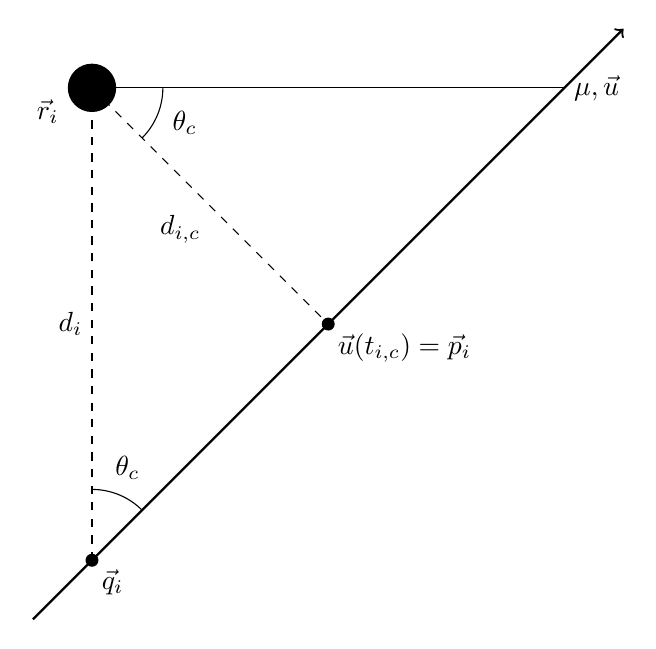
\begin{tikzpicture}[scale=3]
    % Closest point to DOM
    \node [below right] at (0,0) {$\vec{u}(t_{i,c}) = \vec{p}_{i}$};
    \node [below left] at (-0.5, 0.5) {$d_{i,c}$};
    \draw[fill] (0,0) circle [radius=0.025];
    \draw [dashed] (-1,1) -- (0,0);
    % Muon Travel line
    \draw [thick, ->] (-1.25,-1.25) -- (1.25,1.25);
    \node [right] at (1,1) {$\mu, \vec{u}$};
    % Emission point
    \node [below right] at (-1,-1) {$\vec{q}_{i}$};
    \node [above] at (-0.85, -0.7) {$\theta_{c}$};
    \draw[fill] (-1,-1) circle [radius=0.025];
    \draw (-1,-0.7) arc [radius=0.3, start angle=90, end angle=45];
    % DOM
    \node [left] at (-1.1,0.9) {$\vec{r}_{i}$};
    \draw[fill] (-1,1) circle [radius=0.1];
    % Emission Photon
    \node [left] at (-1,0) {$d_{i}$};
    \draw [dashed] (-1,-1) -- (-1,1);
    % Light Wavefront
    \node [right] at (-0.7,0.85) {$\theta_{c}$};
    \draw (-1,1) -- (1,1);
    \draw (-0.7,1) arc [radius=0.3, start angle=0, end angle=-45];
  \end{tikzpicture}
  \caption{Drawing of muon track and Vavilov-Cherenkov Radiation hitting a single DOM where $\vec{r}_{i}$ is the DOM location, $\vec{q}_{i}$ is the emission point of the photon, and $d_{i}$ is the distance the photon travels to the DOM.}
  \label{fig:ghit}
\end{figure}

The next step is to consider the information known about the DOMs. In particular, the direction in which the DOM is facing will determine its angular acceptance giving information on whether or not particular photons can actually reach the DOMs, and the time at which photons are detected. Moreover, light can scatter and may not travel a direct path, so the distance $d_{i}$ also becomes an important parameter to consider. Any sophisticated reconstruction technique will require these parameters to produce reliable results, and hence are important to both understand and compute given a track. Hence, the method for computing these parameters given a DOM position and track will be discussed.

Assuming a track as given in Equation \ref{eq:track}, and that the closest approach position is at $\vec{p}_{i}$ for a DOM at $\vec{r}_{i}$, then it can be easily computed that $d_{i,c} = |\vec{p}_{i} - \vec{r}_{i}|$. Using the closest approach distance,
\begin{equation}\label{eq:dist}
  d_{i} = \frac{d_{i,c}}{\sin\theta_{c}}
\end{equation}
will describe the distance the photon travels. To get the emission point of the photon $\vec{q}_{i}$, it can be seen that $s_{i} = d_{i}/\tan\theta_{c}$ and that the corresponding time would be $t_{s} = s/c$. Then
\begin{equation}
  \vec{q}_{i} = \vec{p}_{i} - ct_{s}\vec{v} = \vec{p}_{i} - s\vec{v}\, ,
\end{equation}
where $\vec{p}_{i} = \vec{u}(t_{i,c}) = \vec{x} + ct_{i,c}\vec{v}$. Due to the photon being emitted before the point of closest approach to the DOM, the distance ($s$) will be negative and thus
\begin{equation}\label{eq:emit}
  \vec{q}_{i} = \vec{x} + (ct_{i,c} - s)\vec{v}\, .
\end{equation}

Now, the emission point and the distance $d_{i}$ from equation \ref{eq:dist} is known. Now, to compute the geometric time, as in the expected photon arrival time at the DOM from the proposed track. To predict this time, a reference along the track is needed, and the vertex $\vec{x}$ is a natural choice for this. Then, 
\begin{equation}
  t_{\text{geo}} = t_{d} + t_{x}
\end{equation}
where
\begin{equation}\label{eq:travel_time}
  t_{d} = \frac{d_{i}}{c_{n}}\, , \hspace{2em} \& \hspace{2em} t_{x} = \frac{(\vec{q}_{i} - \vec{x})\cdot\vec{v}}{c}\, .
\end{equation}
In Equation \ref{eq:travel_time} the former is the time it takes for the emitted photon to travel directly to the DOM, with $c_{n}$ being the group velocity of light in water, and the latter is the time it takes for the muon to travel from the vertex to the emission point. It is important to note that in the second term of Equation \ref{eq:travel_time}, the numerator makes sure that the travel time has the correct value. Since the vertex $\vec{x}$ is not physical, and is mearly a reference point for the purposes of this thesis, it is possible for this location to be after the emission point. In that case, the value $t_{x}$ would have to be negative, and this projection onto the direction vector of the track ensures this. Now, given the time at which the muon is at the vertex, the travel time can be augmented using a shifted $t_{\text{geo}}$ that will now be comparable to the time that the DOM reports, $t_{\text{obs}}$. The parameter of importance then is the residual time, defined as
\begin{equation}
  t_{\text{res}} = t_{\text{obs}} - t_{\text{geo}}\, ,
\end{equation}
as it will vaguely inform of the difference between the geometric guess track and the true track. 

\begin{figure}
  \centering
  \begin{tikzpicture}[scale=3]
    % Origin
    \node [above left] at (-2.5,0.5) {$\mathcal{O}$};
    \draw [fill] (-2.5,0.5) circle [radius=0.05];
    % x and r vector
    \node [below left] at (-1.75,-0.25) {$\vec{x}$};
    \node [above left] at (-1.75,0.75) {$\vec{r}$};
    \node [right] at (-1,-1) {\text{Vertex}};
    \draw [->] (-2.5,0.5) -- (-1.017,-0.982);
    \draw [->] (-2.5,0.5) -- (-1,1);
    % Closest point to DOM
    \node [below left] at (-0.5, 0.5) {$d_{c}$};
    \draw [fill] (0,0) circle [radius=0.025];
    \draw [dashed] (-1,1) -- (0,0);
    % Muon Travel line
    \node [right] at (1,1) {$\mu, \vec{u}$};
    \draw [thick, ->] (-1.25,-1.25) -- (1.25,1.25);
    % Emission point
    \node [below right] at (-0.5,-0.5) {$((\vec{r} - \vec{x})\cdot\vec{v})\vec{v}$};
    \draw [fill] (-1,-1) circle [radius=0.025];
    % DOM
    \node [above] at (-1,1.1) {\text{DOM}};
    \draw [fill] (-1,1) circle [radius=0.1];
    % Emission Photon
    \node [left] at (-1,0) {$\vec{r} - \vec{x}$};
    \draw [->] (-1,-1) -- (-1,1);
  \end{tikzpicture}
  \caption{Drawing of a track with vertex and DOM labeled. The origin here is also marked to emphasize the vector notation and algebra. It is easy enough to see the vector algebra required to get the distance of closest approach through this diagram.}
  \label{fig:dic}
\end{figure}

The next step is to recall all these prior computations rely on the distance of closest approach ($d_{i,c}$) being known. To compute this, geometric considerations with the vectors of the track, the DOM and the vertex need to be considered. To visualize the vector algebra, an origin is introduced from which the vectors can be drawn, in which case Figure \ref{fig:dic} is obtained. The vector pointing to the vertex is $\vec{x}$ and the vector pointing to the DOM is $\vec{r}$, where the indices are dropped for convenience. Then a vector pointing from the vertex to the DOM can be defined by $\vec{r} - \vec{x}$. Next, the projection of this vector along the track direction (which is already a unit vector) is $(\vec{r} - \vec{x})\cdot\vec{v}$. Then, with two sides of a right angle triangle and the third missing side being the length $d_{c}$, so
\begin{equation}
  d_{c} = \sqrt{|\vec{r} - \vec{x}|^{2} - |(\vec{r} - \vec{x})\cdot\vec{v}|^{2}}\, .
\end{equation}

There is now a method of computing $d_{i,c}$, and thus computing $d_{i}$ and $t_{\text{res}}$ for each DOM given a proposed track $\vec{u}(t) = \vec{x} + ct\vec{v}$. It is important here to note the degrees of freedom that parameterizing a track have. The vertex provides four as it is a position in 3-dimensional space with a time. The direction provides two degrees of freedom, as it is a unit vector and can be parameterized using two angles and a unit length radius in spherical coordinates. This gives six parameters in total that need to be computed to uniquely define an infinite track.

A simple way to check that this is working is to plot the arrival times of photons on a single line of detectors whilst varying the direction of the track. Take these detectors to be located starting at the origin and located along the z-axis in space. If a track is traveling such that it intersects the central detector, the arrival times of the photons emitted by this track will take on a well defined shape. Figures \ref{subfig:utime} and \ref{subfig:dtime} show these distributions given particlar track directions with the zenith angle of direction provided. Of the directions given, there is also the special angle of $\theta = \pi/2 \pm \theta_{c}$ which lines up the wavefront with the line of detectors and hence has one of the ``arms'' of the arrival times be populated with coincident hits (they can be slightly off due to approximations). 

\begin{figure}[ht]
  \begin{minipage}[b]{0.48\linewidth}
    \centering
    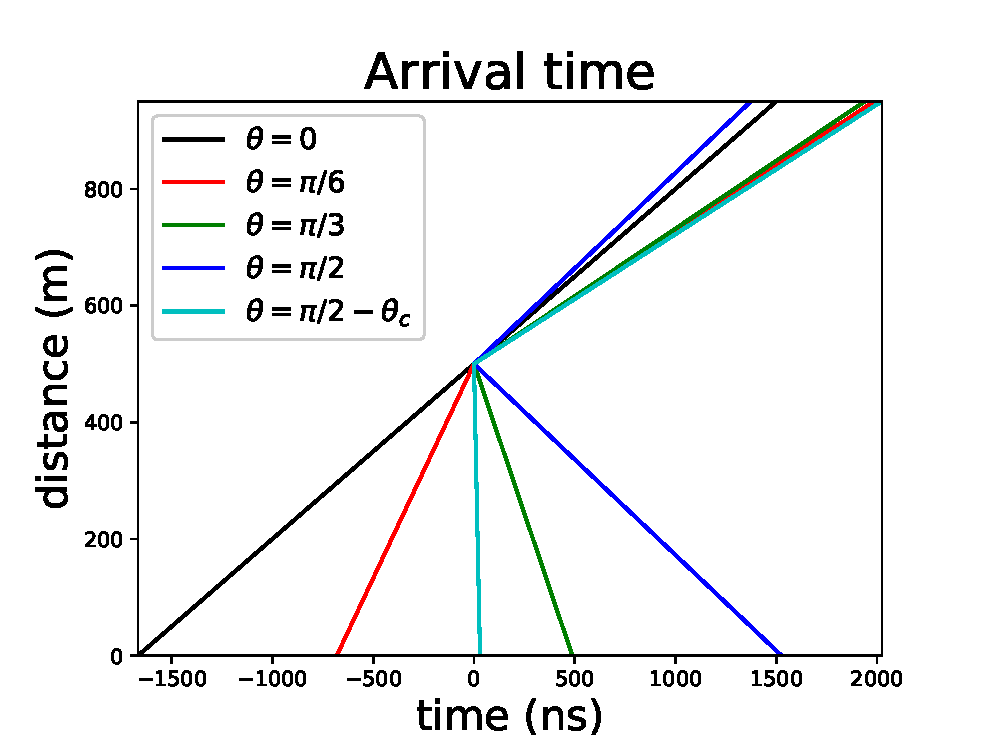
\includegraphics[width=\textwidth]{./Figures/upward_arrival_time.eps}
    \caption{Upward Arrival Time}
    \label{subfig:utime}
  \end{minipage}
  \hspace{0.1cm}
  \begin{minipage}[b]{0.48\linewidth}
    \centering
    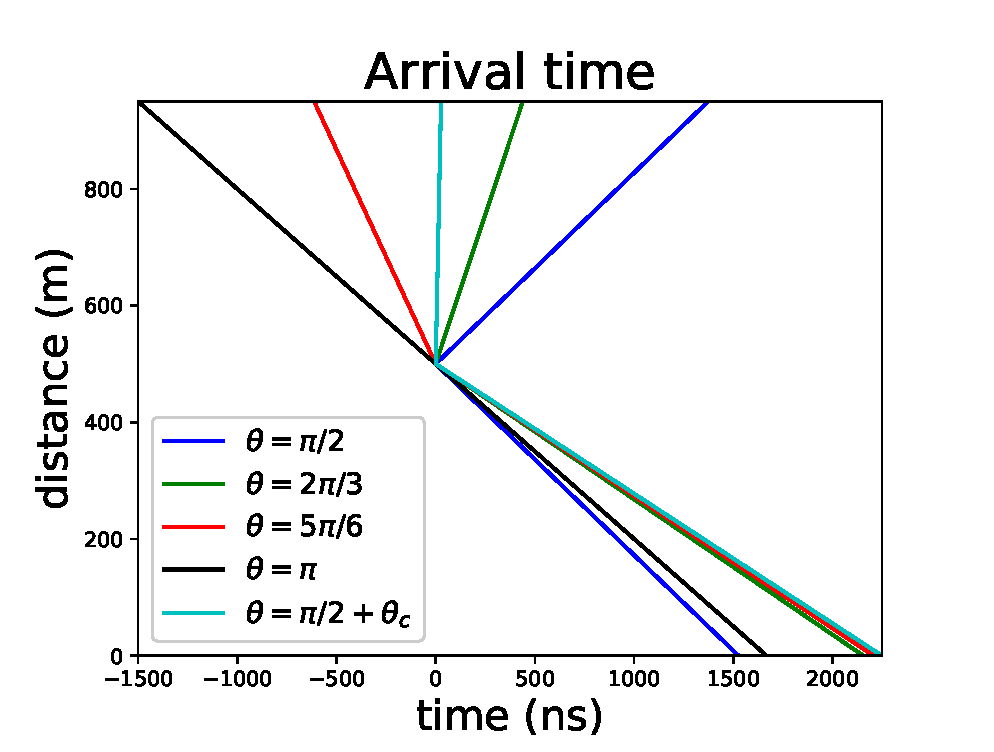
\includegraphics[width=\textwidth]{./Figures/downward_arrival_time.eps}
    \caption{Downward Arrival Time}
    \label{subfig:dtime}
  \end{minipage}
\end{figure}


Now consider different methods for computing these parameters. There are several software techniques that need to be applied before a result can be taken seriously, and usually this pipline begins with a simple and quick initial guess fit. 

\section{Linefit}

Any robust reconstruction method requires an initial guess (generally referred to as a seed) in order to be used, but getting this first guess can be non-trivial. Moreover, reconstruction pipelines can be incredibly sensitive to the initial guess and ensuring the quality of this preliminary fit is difficult in its own right. The standard method for a first guess in such situations is the linear fit. This is a simple track fit that minimizes the $\chi^{2}$ for the observed hits in an event. As such, this fitting technique assumes that all hits on the DOMs are directly on the path of the muon track, which is a reasonable first approximation.

\begin{figure}
  \centering
  \begin{tikzpicture}[scale=5]
    % Drawing the x,y,z-t axis
    \node [right] at (1,0) {$t$};
    \node [above] at (0,1) {$x,y,z$};
    \draw [thick, ->] (0,0) -- (1,0);
    \draw [thick, ->] (0,0) -- (0,1);
    % Drawing the points to be fit
    \draw [fill] (0.1,0.4) circle [radius=0.025];
    \draw [fill] (0.2,0.2) circle [radius=0.025];
    \draw [fill] (0.4,0.4) circle [radius=0.025];
    \draw [fill] (0.6,0.7) circle [radius=0.025];
    \draw [fill] (0.8,0.6) circle [radius=0.025];
    \draw [fill] (0.95,0.85) circle [radius=0.025];
  \end{tikzpicture}
  \caption{Drawing of the position and time space with possible points $(x_{i},y_{i})$ that would be fit.}
  \label{fig:linfit}
\end{figure}

Under these approximations, assume each spatial coordinate independent from the others. Then fit linearly in the projected two dimensional spaces of position and time: $x-t$, $y-t$ and $z-t$, where $t$, the time of the corresponding hit, is the independent variable. This way, the problem is reduced to fitting the equation $y=c_{1}x + c_{0}$ in each position and time space as seen in Figure \ref{fig:linfit}. From here apply $\chi^{2}$ minimization, which in the case of linear data fitting is exactly the method of least squares. In this scenario, if the data points are defined as $(x_{1},y_{1}), \dots, (x_{m},y_{m})$, then the solution that minimizes the $\chi^{2}$ will be
\begin{equation}
  \vec{c} = (X^{T}X)^{-1}X^{T}\vec{y}\, ,
\end{equation}
where
\begin{equation}
  \vec{c} =
  \begin{bmatrix}
    c_{0} \\
    c_{1}
  \end{bmatrix}
  \quad \& \quad
  X =
  \begin{bmatrix}
    1 & x_{1} \\
    1 & x_{2} \\
    \vdots & \vdots \\
    1 & x_{m}
  \end{bmatrix}
  \quad \& \quad
  \vec{y} = 
  \begin{bmatrix}
    y_{1} \\
    y_{2} \\
    \vdots \\
    y_{m}
  \end{bmatrix}\, .
\end{equation}
Once $\vec{c}$ is computed for each position and time space, the vertex position is estimated to be at $(c_{0,x}, c_{0,y}, c_{0,z})$ with direction $(c_{1,x}, c_{1,y}, c_{1,z})$, where the second subscript denotes the spatial component of the data that was used in the fit. 

% Can add charge section (make sure to credit Thomas in statement of originality)
\section{Likelihood}

A more robust technique for reconstructing potential muon tracks is a Maximum Likelihood Estimate \cite{llh_text}. In essence this is a statistically--driven parameter fitting technique that allows for more complex modelling, such as the inclusion of the VC emissions. Specifically, if the $i^{\text{th}}$ DOM observes data $\vec{x_{i}}$, then the probability of observing this data given track parameters $\vec{\theta}$ is described by a probability distribution $p\left(\vec{x_{i}}\bigr\rvert\vec{\theta}\right)$. Since this is true for each DOM in a given event, the likelihood distribution is defined as
\begin{equation}\label{eq:gen_llh}
  \mathcal{L}(\vec{\theta}) = \prod_{i=1}^{n}p\left(\vec{x_{i}}\bigr\rvert\vec{\theta}\right)\, ,
\end{equation}
where the indices are over all $n$ DOMs. The data, $\vec{x}$, can carry information such as the times, charges, and directionality of the hits. The varied parameters, $\vec{\theta}$, carry the information about the track including the direction, the vertex, the vertex time, and the energy. The parameters that maximize the distribution $\mathcal{L}(\vec{\theta})$ are the best estimates for the track given this method.

Finding this maximum is generally non-trivial and a difficult problem. Computational limits motivate using more robust maximization techniques than full parameter searches, and generally these are techniques that use gradient driven methods. Due to this methodology, generally the solution proposed by the MLE is not the global maximum, and is usually a local maximum. The result of the maximization is thus heavily dependent upon the initial conditions and the exact method of fitting.

\subsection{Likelihood Function}

Though the general theory for how the likelihood function will turn out is understood, an explicit form for $p\left(\vec{x_{i}}\bigr\rvert\vec{\theta}\right)$ is still required. This probability function could be made arbitrarily complex by attempting to account for every physical detail, so the assumptions and physical processes that will be modeled need to be stated. The next step would be to account for the scattering and absorption of light using the geometric time and direct distance that the emitted photon would travel before hitting the DOM given a guess track. This seems like a small change, but has large repercussions in the probability distribution describing the data given a hypothesis track. IceCube uses the Pandel function \cite{phd_kai}, which explicitly takes the following form,
\begin{equation}\label{eq:pandel}
  \begin{split}
    p\left(t_{\text{res}}\bigr\rvert\vec{\theta}\right) = & \frac{1}{N(d)}\frac{\tau^{-d/\lambda}\cdot t_{\text{res}}^{d/\lambda - 1}}{\Gamma(d/\lambda)}\cdot \exp\left(-t_{\text{res}}\cdot\left(\frac{1}{\tau} + \frac{c_{\text{medium}}}{\lambda_{a}}\right) - \frac{d}{\lambda_{a}}\right)\, , \\
    N(d) = & e^{-d/\lambda_{a}}\cdot\left(1 + \frac{\tau \cdot c_{\text{medium}}}{\lambda_{a}}\right)^{-d/\lambda}\, ,
  \end{split}
\end{equation}
where $d$ is the photon travel distance, $\lambda$ is the scattering length, $\lambda_{a}$ is the absorption length, $\Gamma(x)$ is the Gamma function, $c_{\text{medium}}$ is the speed of light in water, and $\tau$ is an inverse time parameter for fitting \cite{phd_kai}. Given these parameters, which are physically motivated or fit using simulated data, the Pandel function gives the probability of observing a residual time for a hypothesis track. It is important to note here that $\vec{\theta} = (\vec{v}, \vec{x}, t_{\text{vertex}})$, where we have the track direction, vertex position and vertex time respectively.

The Pandel function favours positive residual times, so much so the probability has varying behavours as $t_{\text{res}}\to 0$. Figure \ref{fig:pandel} shows this behaviour over three different distances over a domain for 300 nanoseconds in residual time. As the distance is increased for the emission point, the probability of observing a photon later than expected increases. This is consistent with the concept of the probability of light being absorbed or scattering increasing as the distance increases. 

\begin{figure}[H]
  \centering
  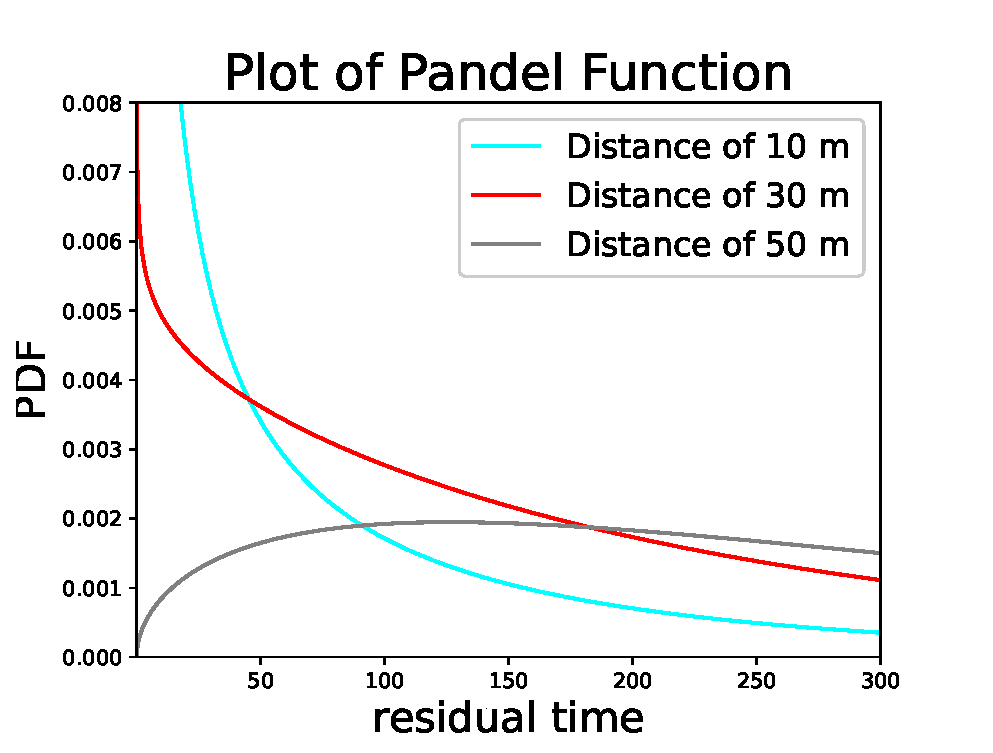
\includegraphics[width=12cm]{./Figures/pandel_plot.eps}
  \caption{A figure showing a plot of the pandel function over 300 nanoseconds with 10 meters, 30 meters and 50 meters of travel for the emitted light. The fit parameters, including $\lambda_{a}$ and $\lambda_{s}$, are fit according to the IceCube parameters as described in \cite{phd_kai}. }
  \label{fig:pandel}
\end{figure}

Theoretically this probability distribution should describe the behaviour of light in water, once the parameters have been fit accordingly. This, however, is not the case practically. The issue arises particularly with the behavour around $t_{\text{res}} = 0$, since in real data there are statistical fluctuations due to uncertainty in data collection. By ignoring the detection step of the process, the Pandel function can't effectively model the data as one would actually observe it, and for this reason the detector error needs to be folded into the function.

The simplest model for detector error is a gaussian, and a known method of folding this error into the Pandel function is a convolution, as done here \cite{conv}. The gaussian width can then be fit and altered to account for any time jittering caused by detection limitations thereby allowing for negative time residuals. If, as in \cite{conv}, the pandel function is reparameterized as $p_{\text{pandel}}(\rho, \xi, t)$ from $p_{\text{pandel}}(\vec{v}, \vec{x}, t)$, then the convolution with a gaussian of mean zero and standard deviation $\sigma$ is given by
\begin{equation}
  \mathcal{F}_{\sigma}(\rho, \xi, t) = \int_{0}^{\infty}\frac{\text{d}x}{\sqrt{2\pi\sigma^{2}}}p(\rho, \xi, x)e^{-(t-x)^{2}/2\sigma^{2}}\, .
\end{equation}
This integral has an exact form \cite{conv},
\begin{equation}\label{eq:exact_cpandel}
  \mathcal{F}_{\sigma}(\rho, \xi, t) = \frac{\rho^{\xi}\sigma^{\xi-1}e^{-t^{2}/2\sigma^{2}}}{2^{(1+\xi)/2}}\left[\frac{_{1}F_{1}(\frac{1}{2}\xi,\frac{1}{2},\frac{1}{2}\eta^{2})}{\Gamma(\frac{1}{2}(\xi+1))} - \sqrt{2}\eta\frac{_{1}F_{1}(\frac{1}{2}(\xi+1),\frac{3}{2},\frac{1}{2}\eta^{2})}{\Gamma(\frac{1}{2}\xi)}\right]\, ,
\end{equation}
where
\begin{equation}
  \eta = \rho\sigma - \frac{t}{\sigma}\, 
\end{equation}
and $_{1}F_{1}$ is the confluent hypergeometric function \cite{conv}. Fortunately $_{1}F_{1}$ is available in multiple computing languages and allows for numerical evaluation of $\mathcal{F}_{\sigma}(\rho, \xi, t)$ \cite{conv}, where there is a plot over an example domain in Figure \ref{fig:cpandel}. This is still non-trivial due to convergence bounds on $_{1}F_{1}$, and as in \cite{conv} approximations for different domains must be used in order to accurately be able to use the entire distance and time domain. For the exact approximations used, refer to \cite{conv}, but the regions that need to be approximated will be discussed. In \cite{conv}, the regions are described using the $\xi$ and $\eta$ parameters, but it is easy enough to translate these to $t$ and $d$. The regions used for this reconstruction are adaped from \cite{conv}.

\begin{figure}[H]
  \centering
  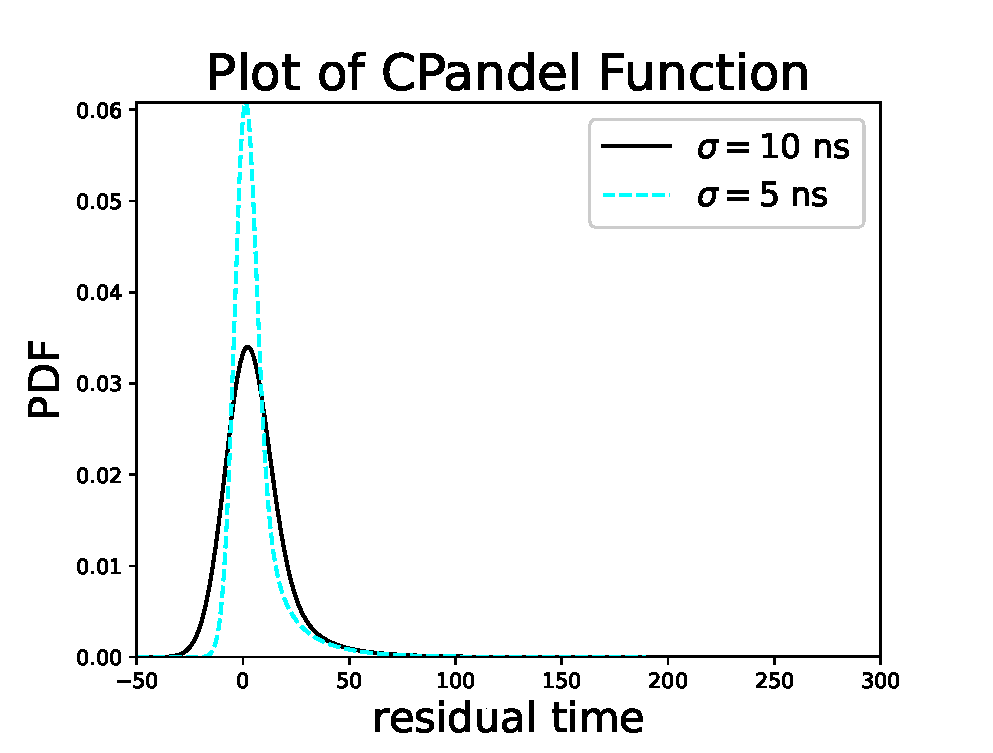
\includegraphics[width=12cm]{./Figures/cpandel_plot.eps}
  \caption{A figure showing a plot of the CPandel function over -50 ns to 300 ns at 50 meters of travel distances for the emitted light. The parameters aside from $\sigma$ are fit according to the simulated data, and we have two plots of $\sigma \in \{5\, \text{ns}, 10\, \text{ns}\}$.}
  \label{fig:cpandel}
\end{figure}

The simplest regions to understand are the unlikely regions. These are the ones in which it is incredibly unlikely to find any events as the residual time is either very positive ($t_{\text{res}} > 3500$ ns), or too negative ($t_{\text{res}} < -25\sigma$ ns). In these regions, independent of distance, these residual times are unphysical and hence heavily penalized by this likelihood. The next region we consider is for $-5\sigma < t_{\text{res}} < 30\sigma$ and $d < 5\lambda_{s}$. This describes the most common region for events to occur, and is within the convergence boundary of the hypergeometric functions. The exact form of the equation, as described in Equation \ref{eq:exact_cpandel}, is the one taken for this region and promotes the general expected behaviour around the peak. The remaining regions are a combination of the possible ranges of distance and time; there are approximations for large $t$ and small $d$, small $t$ and large $d$ and large $t$ and large $d$. These regions each have various approximations associated. The approximations are omitted here but can be found in \cite{conv}.

\subsection{Function Fitting}

In order to use the CPandel distribution, the fitting parameters need to be found such that they match the simulated data. We can see a distribution of the residual times computed over thousands of events in Figure \ref{fig:sim_restime}. Due to the lack of simulated background and noise but instead an artificial Gaussian smearing the resulting distribution is quite smooth and idealized. Moreover, the data is normalized and hence the values on the $y$-axis represent the percentage of the total number of events that fit this criteria.

The data in Figure \ref{fig:sim_restime} is over all distance ranges of the produced light, but the CPandel function clearly depends on the distance as seen in Equation \ref{eq:exact_cpandel}. Thus, it is useful to fit to the simulated data by categorizing over different distance ranges, which can be visualized in similar plots to Figure \ref{fig:sim_restime}. In particular, these plots can be seen in Figures \ref{subfig:res_time_r1}, \ref{subfig:res_time_r3}, \ref{subfig:res_time_r5} and \ref{subfig:res_time_r7}, where the range shifts incrementally upwards over these four figures. With the residual time seperated by distance, it is clear to see the dependence that it has on the distance, and hence the importance of fitting over all of the viable distance ranges of light that will be detected. The prominant feature is a general flattening of the distribution for larger distances, which is expected as light has a higher chance of scattering/being absorbed the further it travels. 

\begin{figure}[H]
  \centering
  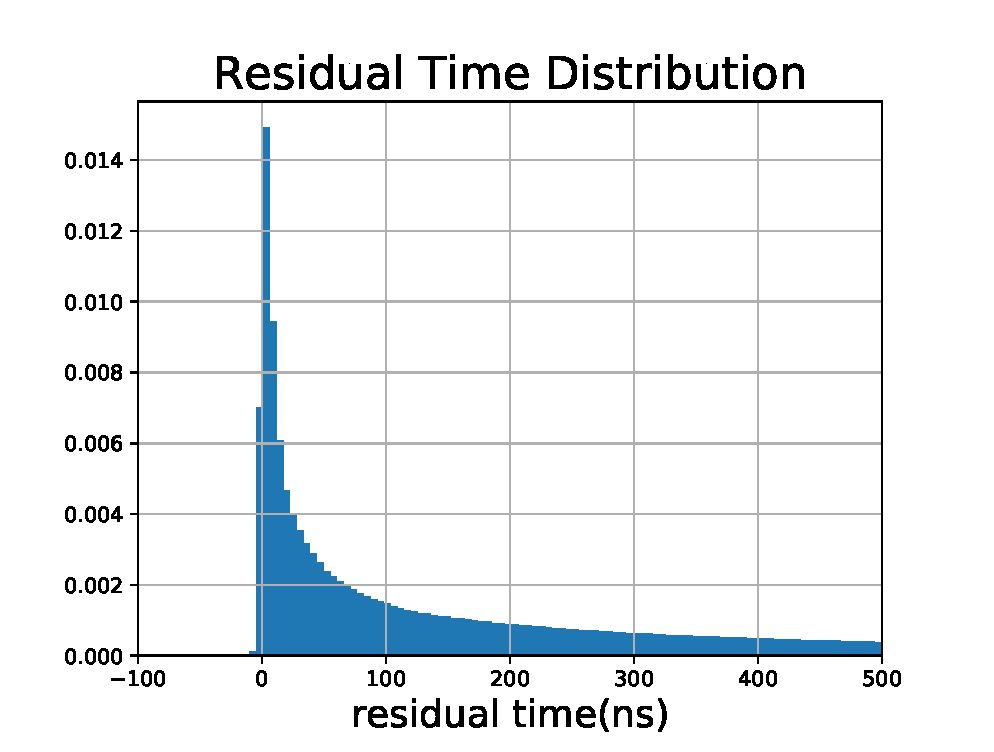
\includegraphics[width=12cm]{./Figures/reco_plots/residual_time_histogram.eps}
  \caption{Normalzied residual time distribution made using simulated events. Here the residual time is computed by comparing the geometric time with the true travel time simulated by the photon propogation software. This does not contain any dark noise or electronic noise and hence is an idealized distribution.}
  \label{fig:sim_restime}
\end{figure}


\begin{figure}[H]
  \begin{minipage}[b]{0.48\linewidth}
    \centering
    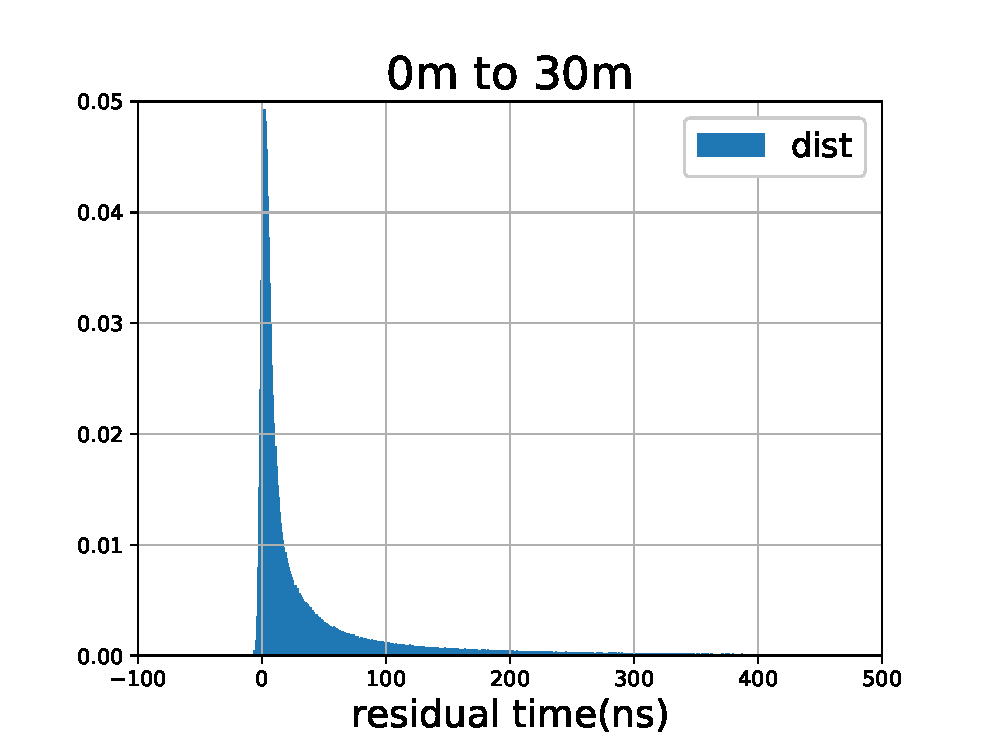
\includegraphics[width=\textwidth]{./Figures/reco_plots/residual_time_hist_r1.eps}
    \caption{Distances from 0 to 30 meters.}
    \label{subfig:res_time_r1}
  \end{minipage}
  \hspace{0.1cm}
  \begin{minipage}[b]{0.48\linewidth}
    \centering
    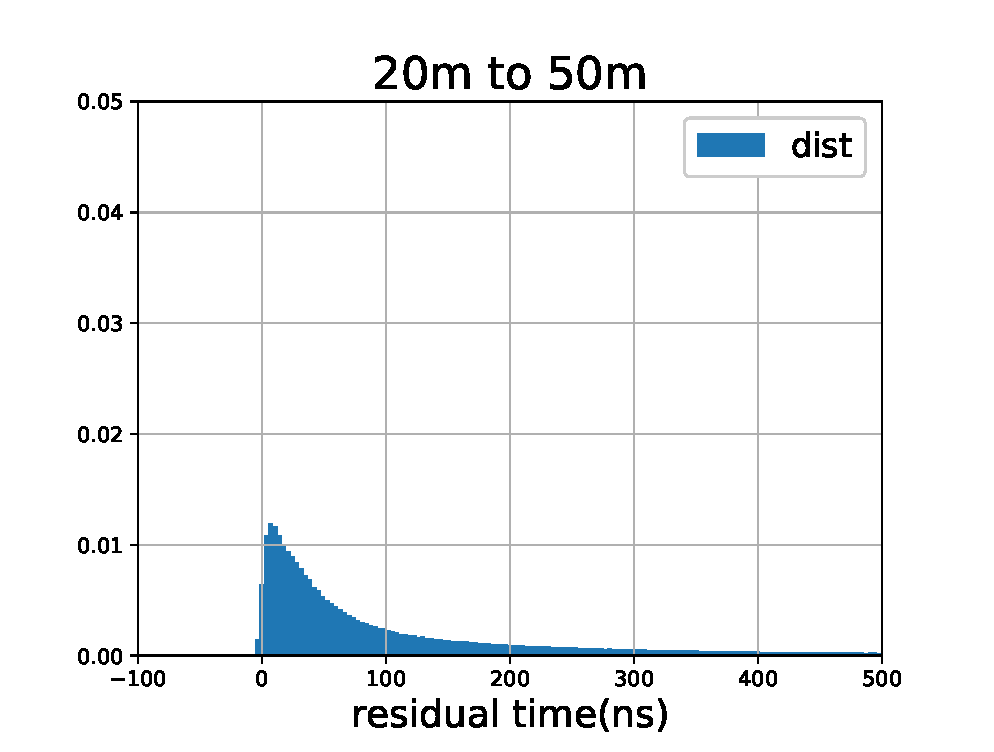
\includegraphics[width=\textwidth]{./Figures/reco_plots/residual_time_hist_r3.eps}
    \caption{Distance from 20 to 50 meters.}
    \label{subfig:res_time_r3}
  \end{minipage}
  \begin{minipage}[b]{0.48\linewidth}
    \centering
    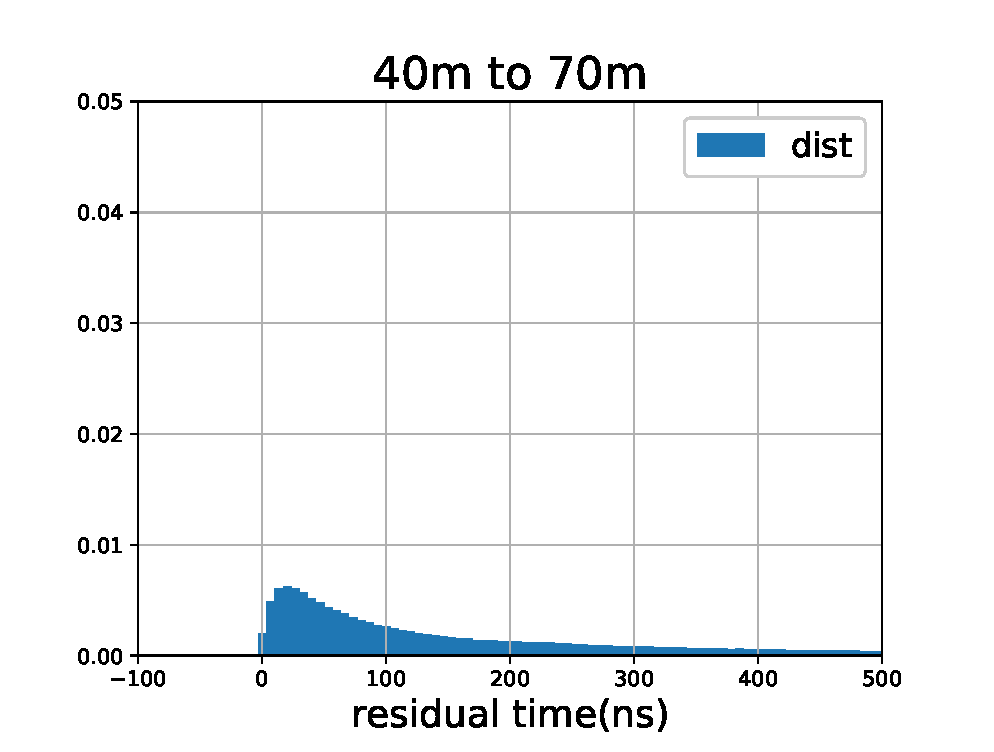
\includegraphics[width=\textwidth]{./Figures/reco_plots/residual_time_hist_r5.eps}
    \caption{Distances from 40 to 70 meters.}
    \label{subfig:res_time_r5}
  \end{minipage}
  \hspace{0.1cm}
  \begin{minipage}[b]{0.48\linewidth}
    \centering
    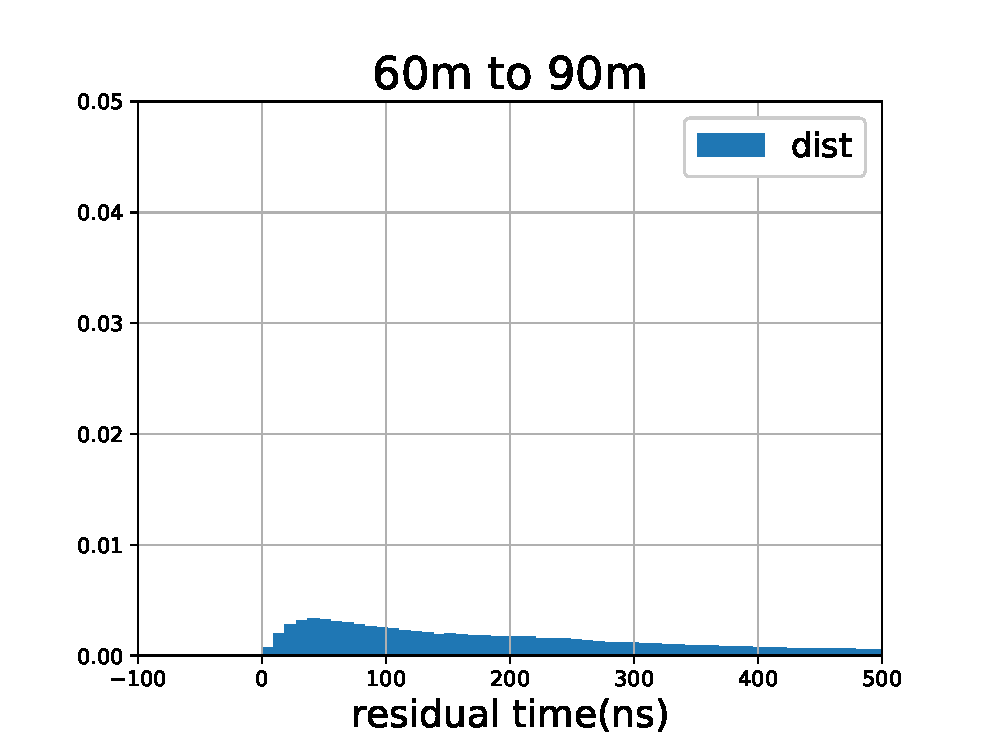
\includegraphics[width=\textwidth]{./Figures/reco_plots/residual_time_hist_r7.eps}
    \caption{Distances from 60 to 90 meters.}
    \label{subfig:res_time_r7}
  \end{minipage}
\end{figure}


\subsection{Other Potential Distributions}

The CPandel isn't the only option for a likelihood distiribution. Another natural choice would be to use real data to emulate a distribution.

\section{Track Fitting}

With the track parameterization understood, a likelihood distribution in the form of the CPandel function, it is now at a point where the reconstruction step can actually take place. As a likelihood, $\mathcal{L}(\vec{\theta})$, for a given track gives a probability, we wish to maximize this function with respect to $\vec{\theta}$. In order to computationally accomplishing this goal, the first step is to utilise a standard method in maximizing likelihoods by taking the logarithm,
\begin{equation}  
  \ell(\vec{\theta}) = \log\left(\mathcal{L}(\vec{\theta})\right)\, .
\end{equation}
As we recall the form for $\mathcal{L}(\vec{\theta})$ in Equation \ref{eq:gen_llh} is a product of probability distributions, then naturally we see
\begin{equation}
  \ell(\vec{\theta}) = \sum_{i=1}^{n}\log\left(p\left(\vec{x_{i}}\bigr\rvert\vec{\theta}\right)\right)\, ,
\end{equation}
which is now a sum rather than a product. This will immediately be more useful as computationally it is easier to take a sum then a product. Another point to note is that generally one finds the minimums of functions rather than maximums purely due to convention, and so generally the minima of $-\ell(\vec{\theta})$ is what is computed.

For the actual minimization process, the common method is to use a simplex based technique \cite{simplex}. This method, sometimes referred to as the Nedler-Mead algorithm, is powerful for finding local minima of multi-parameter systems and uses an approach that does not rely on derivatives. The benefit is that this method is relatively straight forward and easily implemented. A more robust technique is to use a gradient based approach, such as the nonlinear conjugate gradient method \cite{gradient}, which uses a gradient to determine the direction in which the minimizer will head. The benefit to this latter approach is that it is more consistent and reliable in finding the minima.

Ultimately the choice of minimization technique is case dependent and can vary. Both of these are compared in the analysis.

\section{Corrections}

Through some testing and debugging, it was found there were some manual corrections and changes that had to be made to observe an improvement in the likelihood reconstruction. These changes included reparameterizing the problem into a spherical coordinate-like form, and an extra penalty on the likelihood for negative residual values.

\subsection{Reparameterizing}

Due to the seed for the likelihood fit being parameters resulting from the linear fit, the resultant minimization can vary depending upon how well the original fit does. A flaw of the linear fit method is that the vertex fit is not physically meaningful, and doesn't serve any other purpose in this initial fitting technique. This can occasionally result in a vertex that is very far away from the director, which can have drastic effects on the minimization. In particular, the further the vertex is from the detector the more sensitive the minimizer is to changes in the direction azimuth and zenith angles. This can impede the minimization process, and cause the minimizer to miss even local minimas.

To avoid these potential issues, the problem was reparameterized from $\vec{\theta} = (\theta, \phi, \vec{x}, t)$ to $\vec{\theta} = (\theta, \phi, \vartheta, \varphi, t)$. The new $\vartheta$ and $\varphi$ refer to the zenith and azimuth angles that point to the vertex at a fixed radius $r$ related to the size of the detector. Fixing $r$ determines a sphere around the center of the detector, and the intersection of the track with that sphere is determined and the new vertex is determined to be the first point that intersects the sphere, hwhich allows for computation of these new angles. If the line does not intersect the sphere, the event is determined to be outside the detector and would be disregarded in event cleaning anyways. 

\subsection{Extra Penalty}

As the likelihood function represents the ideal residual time distribution, the goal of the likelihood method is to generally push the distribution towards the CPandel distribution. This is a vague approximation of how the likelihood method actually works, but it motivates penalizing negative residual values even more. Ocassionaly the minimization process won't find a distribution that fits the CPandel well, and in these cases adding an extra artificial presence to nudge the residual time distribution in the right direction can improve the fit.

Though this solution works, it is inherently temporary and is a band-aid method to force the likelihood minimization to behave the way we want. Ideally the likelihood distribution would be robust enough to correctly push the minimization in the correct direction without this manual push. 
